%
% This is a borrowed LaTeX template file for lecture notes for CS267,
% Applications of Parallel Computing, UCBerkeley EECS Department.
% Now being used for CMU's 10725 Fall 2012 Optimization course
% taught by Geoff Gordon and Ryan Tibshirani.  When preparing 
% LaTeX notes for this class, please use this template.
%
% To familiarize yourself with this template, the body contains
% some examples of its use.  Look them over.  Then you can
% run LaTeX on this file.  After you have LaTeXed this file then
% you can look over the result either by printing it out with
% dvips or using xdvi. "pdflatex template.tex" should also work.
%

\documentclass[twoside]{article}
\setlength{\oddsidemargin}{0.25 in}
\setlength{\evensidemargin}{-0.25 in}
\setlength{\topmargin}{-0.6 in}
\setlength{\textwidth}{6.5 in}
\setlength{\textheight}{8.5 in}
\setlength{\headsep}{0.75 in}
\setlength{\parindent}{0 in}
\setlength{\parskip}{0.1 in}

%
% ADD PACKAGES here:
%

\usepackage{amsmath,amsfonts,graphicx}
\usepackage{tikz}
\usetikzlibrary{automata,positioning}
%
% The following commands set up the lecnum (lecture number)
% counter and make various numbering schemes work relative
% to the lecture number.
%
\newcounter{lecnum}
\renewcommand{\thepage}{\thelecnum-\arabic{page}}
\renewcommand{\thesection}{\thelecnum.\arabic{section}}
\renewcommand{\theequation}{\thelecnum.\arabic{equation}}
\renewcommand{\thefigure}{\thelecnum.\arabic{figure}}
\renewcommand{\thetable}{\thelecnum.\arabic{table}}

%
% The following macro is used to generate the header.
%
\newcommand{\lecture}[4]{
   \pagestyle{myheadings}
   \thispagestyle{plain}
   \newpage
   \setcounter{lecnum}{#1}
   \setcounter{page}{1}
   \noindent
   \begin{center}
   \framebox{
      \vbox{\vspace{2mm}
    \hbox to 6.28in { {\bf CPSC 313: Introduction to Computability
	\hfill Fall 2016} }
       \vspace{4mm}
       \hbox to 6.28in { {\Large \hfill Lecture #1: #2  \hfill} }
       \vspace{2mm}
       \hbox to 6.28in { {\it Lecturer: #3 \hfill Scribe: #4} }
      \vspace{2mm}}
   }
   \end{center}
   \markboth{Lecture #1: #2}{Lecture #1: #2}


}
%
% Convention for citations is authors' initials followed by the year.
% For example, to cite a paper by Leighton and Maggs you would type
% \cite{LM89}, and to cite a paper by Strassen you would type \cite{S69}.
% (To avoid bibliography problems, for now we redefine the \cite command.)
% Also commands that create a suitable format for the reference list.
\renewcommand{\cite}[1]{[#1]}
\def\beginrefs{\begin{list}%
        {[\arabic{equation}]}{\usecounter{equation}
         \setlength{\leftmargin}{2.0truecm}\setlength{\labelsep}{0.4truecm}%
         \setlength{\labelwidth}{1.6truecm}}}
\def\endrefs{\end{list}}
\def\bibentry#1{\item[\hbox{[#1]}]}

%Use this command for a figure; it puts a figure in wherever you want it.
%usage: \fig{NUMBER}{SPACE-IN-INCHES}{CAPTION}
\newcommand{\fig}[3]{
			\vspace{#2}
			\begin{center}
			Figure \thelecnum.#1:~#3
			\end{center}
	}
% Use these for theorems, lemmas, proofs, etc.
\newtheorem{theorem}{Theorem}[lecnum]
\newtheorem{lemma}[theorem]{Lemma}
\newtheorem{proposition}[theorem]{Proposition}
\newtheorem{claim}[theorem]{Claim}
\newtheorem{corollary}[theorem]{Corollary}
\newtheorem{definition}[theorem]{Definition}
\newenvironment{proof}{{\bf Proof:}}{\hfill\rule{2mm}{2mm}}

% **** IF YOU WANT TO DEFINE ADDITIONAL MACROS FOR YOURSELF, PUT THEM HERE:

\newcommand\E{\mathbb{E}}

\begin{document}
%FILL IN THE RIGHT INFO.
%\lecture{**LECTURE-NUMBER**}{**DATE**}{**LECTURER**}{**SCRIBE**}
\lecture{19}{Midterm Review}{Dr. Catalin Dohotaru}{Shane Sims}
%\footnotetext{These notes are partially based on those of Nigel Mansell.}

% **** YOUR NOTES GO HERE:

% Some general latex examples and examples making use of the
% macros follow.  
%**** IN GENERAL, BE BRIEF. LONG SCRIBE NOTES, NO MATTER HOW WELL WRITTEN,
%**** ARE NEVER READ BY ANYBODY.


\section{Examples: Regular Expression} % Don't be this informal in your notes!

Give a regular expression for each of the following languages:

\begin{enumerate}
\item The language of all strings containing at least two 0s and at least a 1.\newline

\textbf{Solution:} The possible patterns of the required symbols are: $001, 010 \text{ and } 100$. In between we can have any string, $(0 + 1)^*$. Then any string in this language can be obtained from the regular expression to follow, where each of the three parts correspond to the three possibilities just noted:\newline

$(0 + 1)^*0(0 + 1)^*0(0 + 1)^*1(0 + 1)^*+ (0 + 1)^*0(0 + 1)^*1(0 + 1)^*0(0 + 1)^* + (0 + 1)^*1(0 + 1)^*0(0 + 1)^*0$\newline
\item The language of all strings in which the number of 0s and the number of 1s are not both odd.\newline

\textbf{Solution:} Notice that the requirement that the number of 0s and 1s are not both odd means that either the number of 0s are even, or the number of 1s is even. Then we have the following regular expression: \newline

$1^*(01^*01^*)^*+0^*(10^*10^*)^*$\newline
\item The language of all strings in which every run of 0s has a length of at least 3.\newline

\textbf{Solution:} $(1+0000^*)^*)$
\end{enumerate}

\section{Examples: Questions concerning NFAs}

\begin{enumerate}
\item Show that if $N$ is an NFA that recognizes a language $L$, swapping the accept and non-accept states in $N$ does not necessarily give a new NFA that recognizes $\bar{L}$, as was possible in the case concerning DFAs.\newline

\textbf{Solution:}\newline

\begin{tikzpicture}[shorten >=1pt,node distance=2cm,on grid,auto]
   \node[state, initial] (q_0){$q_0$};
   \node[state, accepting] (q_1) [right=of q_0] {$q_1$};
    \
    \path[->] 
    (q_0) edge  node {0,1} (q_1)
        edge [loop above] node {0} ()
    (q_1);
    
     \node [below=1cm, align=flush center,text width=8cm] at (q_0)
        {
            $N$
        };
\end{tikzpicture}
\qquad
\begin{tikzpicture}[shorten >=1pt,node distance=2cm,on grid,auto]
   \node[state, initial, accepting] (q_0){$q_0$};
   \node[state] (q_1) [right=of q_0] {$q_1$};
    \
    \path[->] 
    (q_0) edge  node {0,1} (q_1)
        edge [loop above] node {0} ()
    (q_1);
    
     \node [below=1cm, align=flush center,text width=8cm] at (q_0)
        {
            $N'$
        };
\end{tikzpicture}
Notice that both NFAs accept $0$.\newline

\item Prove that the following language is regular:\newline
$L = $ \{$w \in$ \{$0, 1$\}$| w$ contains at most one occurrence of the substring 00\}\newline
For example, the string 000 has two occurrences of 00.\newline

\textbf{Solution: } The two primary methods we have seen so far to prove that a language is regular, is to provide a finite automation or a regular expression for the language. In this case both of these methods prove difficult. A simpler solution is to make a finite automation (DFA or NFA) for the compliment of $L$, recalling that once we have done this, we can simply flip the accept and non-accept states, the result being a finite automation for $L$.\newline
We observe that $\bar{L} = $\{$w\in$\{0,1\}*$| w$ contains at least two occurrences of 00\}. We create the following NFA for this language: \newline

\begin{tikzpicture}[shorten >=1pt,node distance=2cm,on grid,auto]
   \node[state, initial] (q_0){$q_0$};
   \node[state] (q_1) [right=of q_0] {$q_1$};
   \node[state] (q_2) [right=of q_1] {$q_2$};
   \node[state, accepting] (q_3) [right=of q_2] {$q_3$};
   \node[state] (q_4) [below=of q_1] {$q_4$};
   \node[state] (q_5) [right=of q_4] {$q_5$};
   \node[state] (q_6) [right=of q_5] {$q_6$};
   \node[state, accepting] (q_7) [right=of q_6] {$q_7$};
    \
    \path[->] 
    (q_0) edge node {0} (q_1)
    (q_0) edge node {0} (q_4)
        edge [loop above] node {0,1} ()
    (q_1) edge node {0} (q_2)
    (q_2) edge node {0} (q_3)
    (q_3) edge [loop above] node {0,1}()
    (q_4) edge node {0} (q_5)
    (q_5) edge node {0} (q_6)
    		edge [loop above] node {0,1} ()
	(q_6) edge node {0} (q_7)
    (q_7) edge [loop above] node {0,1}();
\end{tikzpicture}
\newline
\item Let $L \subseteq \Sigma^*$ be an arbitrary regular language. Prove that the following languages are regular:
\begin{enumerate}
\item PREFMIN(L) $=$ \{ $xy\in L | x\in L \leftrightarrow y = \epsilon$\}
\item SUFMIN(L) $=$ \{$xy\in L | y\in L \leftrightarrow x = \epsilon$\}
\end{enumerate}

\begin{enumerate}
\item \textbf{Solution:} We can reformulate the language as:  PREFMIN(L) $=$ \{ $w\in L |$ no proper prefix of $w$ is a member of $L$\}.\newline
Ex: If $L = \left\{ 0110, 00, 0010 \right\}$, then PREFMIN(L) $= \left\{ 0110, 00 \right\}$. Notice that $0010$ is not a member of the later language because a prefix of this string, namely $00$, is already a member of $L$. We see that example NFAs for $L$ and PREFMIN(L) are respectively as follows:\newline

\begin{tikzpicture}[shorten >=1pt,node distance=2cm,on grid,auto]
   \node[state, initial] (q_0){$q_0$};
   \node[state] (q_1) [right=of q_0] {$q_1$};
   \node[state] (q_2) [right=of q_1] {$q_2$};
   \node[state, accepting] (q_3) [right=of q_2] {$q_3$};
   \node[state, accepting] (q_4) [right=of q_3] {$q_4$};
   \node[state, accepting] (q_5) [below=of q_2] {$q_5$};
   \node[state] (q_6) [right=of q_5] {$q_6$};
    \
    \path[->] 
    (q_0) edge node {0} (q_1)
    (q_1) edge node {1} (q_2)
    (q_1) edge node {0} (q_5)
    (q_2) edge node {1} (q_3)
    (q_3) edge node {0} (q_4)
    (q_5) edge node {1} (q_6)
    (q_6) edge node {0} (q_4);
\end{tikzpicture}
\newline
\newline
\begin{tikzpicture}[shorten >=1pt,node distance=2cm,on grid,auto]
   \node[state, initial] (q_0){$q_0$};
   \node[state] (q_1) [right=of q_0] {$q_1$};
   \node[state] (q_2) [right=of q_1] {$q_2$};
   \node[state, accepting] (q_3) [right=of q_2] {$q_3$};
   \node[state, accepting] (q_4) [right=of q_3] {$q_4$};
   \node[state, accepting] (q_5) [below=of q_2] {$q_5$};
   \node[state] (q_6) [right=of q_5] {$q_6$};
    \
    \path[->] 
    (q_0) edge node {0} (q_1)
    (q_1) edge node {1} (q_2)
    (q_1) edge node {0} (q_5)
    (q_2) edge node {1} (q_3)
    (q_3) edge node {0} (q_4)
    (q_6) edge node {0} (q_4);
\end{tikzpicture}
\newline
Now we can see that a NFA recognizing PREFMIN(L), we simply remove all transitions in the DFA for L that originate from a final state.\newline
 So if we let $M = (Q, \Sigma, \delta, q_0, F)$ be a DFA recognizing $L$, we construct an NFA, N, recognizing PREFMIN(L): $N = (Q, \Sigma, \delta', q_0, F)$, where\newline
 \begin{displaymath}
   \delta'(q,a) = \left\{
     \begin{array}{lr}
       \delta(q,a) & : q \notin F\\
       \emptyset & : q \in F
     \end{array}
   \right.
\end{displaymath}
\item \textbf{Solution:} Similarly, we reformulate the language as:  SUFMIN(L) $=$ \{ $w\in L |$ no proper suffix of $w$ is a member of $L$\}.\newline
Ex: If $L = \left\{ 10, 010, 100 \right\}$, then SUFMIN(L) $= \left\{ 10, 100 \right\}$. Notice that $L^R = \left\{ 01, 010, 001 \right\}$, and PREFMIN($L^R$) $= \left\{ 01, 001 \right\}$.\newline
In general, SUFMIN(L) = $(\text{PREFMIN}(L^R))^R$.\newline
 $(\text{SUFMIN(L)})^R =$ \{$y^Rx^R\in L^R | y^R\in L^R \leftrightarrow x^R = \epsilon$\}.
 
\end{enumerate}
\end{enumerate}




% **** THIS ENDS THE EXAMPLES. DON'T DELETE THE FOLLOWING LINE:

\end{document}





